% SecondChance -- project report
% Compile on Overleaf. Upload the PNGs from shelter/results/plots/ into a
% folder named "figures" next to this file (or upload the whole shelter folder).
\documentclass[11pt,a4paper]{article}

\usepackage[margin=2.4cm]{geometry}
\usepackage[T1]{fontenc}
\usepackage{lmodern}
\usepackage{microtype}
\usepackage{booktabs}
\usepackage{array}
\usepackage{enumitem}
\usepackage{titlesec}
\usepackage{xcolor}
\usepackage{graphicx}
\usepackage{caption}
\usepackage[hidelinks]{hyperref}

\graphicspath{{figures/}{../results/plots/}{shelter/results/plots/}}

\definecolor{jiitblue}{RGB}{23,54,93}
\titleformat{\section}{\color{jiitblue}\normalfont\Large\bfseries}{\thesection.}{0.6em}{}[\vspace{-6pt}\rule{\textwidth}{0.6pt}]
\titleformat{\subsection}{\normalfont\large\bfseries}{\thesubsection}{0.6em}{}
\setlist{nosep,leftmargin=1.4em}
\renewcommand{\arraystretch}{1.25}
\captionsetup{font=small,labelfont=bf}
\newcolumntype{L}[1]{>{\raggedright\arraybackslash}p{#1}}
\newcolumntype{R}[1]{>{\raggedleft\arraybackslash}p{#1}}

\begin{document}
\pagestyle{empty}

\begin{center}
\vspace*{1.2cm}
{\color{jiitblue}\Large\bfseries JAYPEE INSTITUTE OF INFORMATION TECHNOLOGY}\\[4pt]
{\large Noida, Uttar Pradesh}\\[2.0cm]

{\large P\,R\,O\,J\,E\,C\,T\quad R\,E\,P\,O\,R\,T}\\[4pt]
{\large Machine Learning and Data Mining}\\[1.0cm]

\rule{0.62\textwidth}{0.8pt}\\[0.7cm]
{\color{jiitblue}\Huge\bfseries SecondChance}\\[0.7cm]
{\large Mining Attribute Bias in Animal Shelter Outcomes with\\
Association Rules and Density-Based Clustering}\\[0.6cm]
\rule{0.62\textwidth}{0.8pt}

\vfill
\begin{minipage}[t]{0.45\textwidth}
\raggedright
{\color{jiitblue}\bfseries Submitted to:}\\[6pt]
Dr. Ashish Mishra
\end{minipage}
\hfill
\begin{minipage}[t]{0.45\textwidth}
\raggedleft
{\color{jiitblue}\bfseries Submitted by:}\\[6pt]
\begin{tabular}{@{}lr@{}}
Sambhav Ghildiyal & 23803005 \\
Aniket Pandey & 23803008 \\
Aditya Bansal & 23803009 \\
Mudit Maheshwari & 23803017 \\
\end{tabular}
\end{minipage}

\vspace{1.2cm}
November 2026
\end{center}

\newpage
\pagestyle{plain}
\setcounter{page}{1}
\tableofcontents
\newpage

%% ==================================================================
\section*{Abstract}
\addcontentsline{toc}{section}{Abstract}
\rule{\textwidth}{0.6pt}\vspace{4pt}

Municipal animal shelters triage under permanent capacity pressure, and
practitioners hold strong beliefs about what decides an animal's fate --- that
black animals are passed over, that bully-breed labels are disqualifying, that
senior animals are unadoptable. These beliefs shape policy and are rarely
measured at scale.

We analyse \textbf{162{,}461} dog and cat outcome events published by Austin
Animal Center between October 2013 and May 2025, joined to the corresponding
intake records at 99.1\,\% coverage. Using only algorithms taught in the course
--- Apriori, decision tree, Naive Bayes, KNN, SVM, a backpropagation neural
network, K-Means, K-Medoids, hierarchical, DBSCAN and OPTICS --- we find:

\begin{enumerate}[label=(\roman*)]
  \item \textbf{``Black dog syndrome'' is not supported.} Black dogs are adopted
        \emph{more} often than other dogs (+2.77 pp); black cats slightly less
        (--2.25 pp). After direct standardisation, white animals fare worst.
  \item \textbf{Age and breed label dominate.} Senior dogs are adopted 23.66 pp
        less often; pit bull type dogs wait a median of 10.0 days against 5.3.
  \item \textbf{Atypical animals fare worse.} Animals labelled noise by DBSCAN
        and OPTICS --- identified with no labels at all --- are euthanised at
        2.57$\times$ and 3.11$\times$ the rate of clustered animals.
  \item \textbf{Association rules and decision trees agree on rules but not on
        attributes.} Two thirds of tree leaves have a matching mined rule, yet
        the attribute rankings correlate at $\rho = 0.055$. The tree never
        splits on colour; Apriori reports colour freely. This is the difference
        between what is \emph{sufficient} and what is \emph{associated}, and it
        explains the colour result by a third independent route.
  \item \textbf{Honest evaluation costs accuracy.} Mean MCC falls from 0.308
        under a random split to 0.258 under a temporal holdout.
\end{enumerate}

%% ==================================================================
\section{Introduction}

Shelter intake exceeds adoption capacity almost everywhere, so triage is
unavoidable and its consequences are terminal. Staff decide which animals
receive foster placement, promotion or extended holding time, largely guided by
experience and folklore rather than measurement.

The most widely cited of these beliefs is ``black dog syndrome'': the claim that
dark-coated animals wait longer and are adopted less often. It is believed
strongly enough to drive operational policy --- shelter photography guidelines,
the removal of breed labels from kennel cards --- yet reported findings in the
literature are mixed, and most studies cover a single shelter over a short
window.

A public dataset of 173{,}775 outcomes spanning more than a decade makes the
question tractable. We ask two things:

\begin{enumerate}[label=\textbf{Q\arabic*.}]
  \item Which attributes actually determine an animal's outcome, and by how
        much, once the remaining attributes are controlled for?
  \item Can an adverse outcome be anticipated early enough to act on, using only
        what is recorded when the animal enters the shelter?
\end{enumerate}

Interpretability is a requirement here rather than a preference. A shelter
manager cannot act on a risk score; they need the reason, because the reason is
what suggests the intervention. This makes decision trees and association rules
the appropriate instruments, and makes the comparison against less transparent
models a trade-off to measure rather than a formality.

%% ==================================================================
\section{Dataset}

\begin{center}
\begin{tabular}{@{}L{3.3cm}L{12.0cm}@{}}
\toprule
\textbf{Property} & \textbf{Austin Animal Center} \\
\midrule
Outcomes & 173{,}775 events, Oct 2013 -- May 2025 \\
Intakes & 173{,}812 events; joined on Animal ID at \textbf{99.1\,\%} \\
Analysed & \textbf{162{,}461} dog and cat outcome events \\
Features & animal type, breed (3{,}010 free-text strings), colour (663), sex and
sterilisation status, age, intake type, intake condition \\
Label & Adoption 83{,}866 (51.6\,\%); Transfer 46{,}668 (28.7\,\%); Return to
Owner 25{,}466 (15.7\,\%); Euthanasia 4{,}704 (2.9\,\%); Other 1{,}757 (1.1\,\%) \\
Access & Two public CSVs, no account or API key, 21\,MB and 26\,MB \\
\bottomrule
\end{tabular}
\end{center}

\begin{figure}[htbp]
\centering
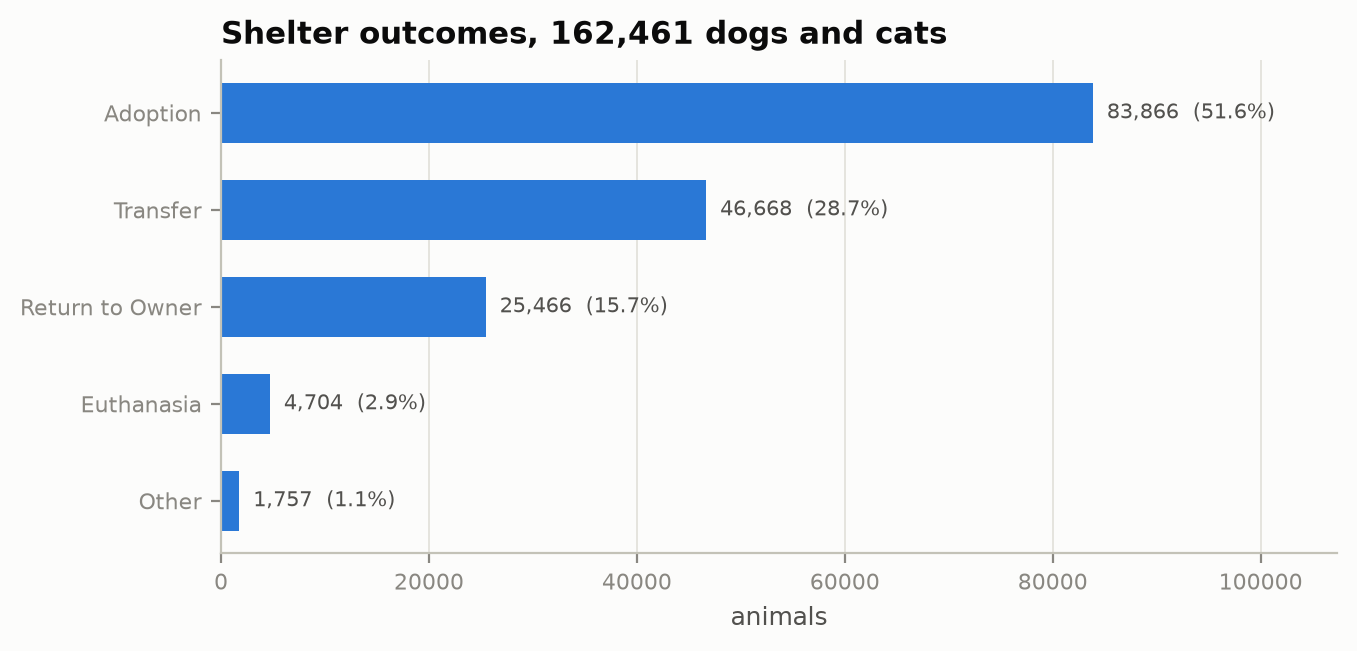
\includegraphics[width=0.78\textwidth]{01-outcomes.png}
\caption{Outcome distribution across 162{,}461 dog and cat events. Adoption
accounts for just over half of all outcomes, which is why accuracy is an
uninformative metric here (Section~\ref{sec:classification}).}
\end{figure}

Scoping to dogs and cats retains 94\,\% of records and removes wildlife
intakes --- bats, chiefly --- for which ``adoption'' is not a meaningful
outcome. This also lowers the euthanasia share from 6.2\,\% to 2.9\,\%, because
much of the shelter's euthanasia is wildlife.

%% ==================================================================
\section{Preprocessing}

\subsection{Three properties of the data that shape the method}

\textbf{Mixed timezone offsets.} The \texttt{DateTime} column carries mixed UTC
offsets in both files. Parsed naively, comparing timestamps raises
\texttt{can't compare offset-naive and offset-aware datetimes}; parsing as UTC
is required.

\textbf{Animals return.} Roughly 10\,\% of Animal IDs occur more than once in
the Intakes file. A one-row-per-animal merge is therefore wrong. The join is
performed per \emph{outcome event}, matched to the most recent intake at or
before that outcome (\texttt{pandas.merge\_asof}, backward direction). Length of
stay is the difference; no negative stays result, which is the check that the
direction is correct.

\textbf{The obvious feature leaks the label.} \texttt{Sex upon Outcome} encodes
sterilisation status, and shelters routinely sterilise animals \emph{as part of}
preparing them for adoption. A model given this feature learns that sterilised
animals get adopted, which is circular. Every feature is therefore taken from
the \textbf{intake} record, which is also what predicting at intake honestly
means.

\subsection{Normalisation}

Breed strings are normalised by an ordered rule list: the \texttt{Mix} suffix
becomes a separate flag, slash-delimited crosses are reduced to the first
component, and the remainder is mapped to one of 50 breed groups.
Locally-specific names are folded correctly --- ``queensland heeler'' and ``blue
heeler'' are the same breed as the Australian cattle dog, and the free-text
field uses all three. \textbf{98.9\,\%} of records land in a named group.

Colour strings are split into a primary colour and a pattern keyword (tabby,
brindle, tricolor, point, merle), then mapped to ten colour groups. Age strings
are parsed to days and bucketed into five bands. The combined sex field is split
into sex and sterilisation status, which are distinct predictors.

Every mapping is written to \texttt{results/tables/normalisation\_map.csv} so
the transformation is auditable rather than implicit.

%% ==================================================================
\section{Methodology}

\begin{center}
\small
\begin{tabular}{@{}L{3.6cm}L{5.4cm}L{5.8cm}@{}}
\toprule
\textbf{Question} & \textbf{Technique} & \textbf{Why this one} \\
\midrule
What goes with what? & Apriori, FP-Growth & transactions are attribute sets;
rules ranked by lift \\
What can we predict? & Decision tree, Naive Bayes, KNN, SVM, MLP & two
protocols, identical test set \\
What groups exist? & K-Means, K-Medoids, Hierarchical, DBSCAN, OPTICS & Hamming
dissimilarity on categorical attributes \\
Who is at risk unlabelled? & DBSCAN / OPTICS noise & density, not supervision \\
Does colour matter? & direct standardisation & controls confounding without
regression \\
\bottomrule
\end{tabular}
\end{center}

\subsection{Why Hamming, and why K-Means is included to lose}
\label{sec:hamming}

Every attribute is categorical, so Euclidean distance is not meaningful. The
appropriate dissimilarity is \textbf{Hamming}: the fraction of the eleven
attributes on which two animals differ. Because there are eleven attributes it
takes only twelve distinct values, and far from being a limitation this makes
the neighbourhood radius directly interpretable:

\begin{center}
$\texttt{eps} = 2/11 \quad\equiv\quad$ \textit{``animals differing in at most two
attributes are neighbours''}
\end{center}

K-Medoids, hierarchical clustering, DBSCAN and OPTICS all accept a precomputed
dissimilarity matrix, so all four run on Hamming. \textbf{K-Means cannot}: it
computes means, which requires Euclidean geometry, and the mean of categorical
vectors is not an animal. It is included deliberately, on one-hot data, as the
contrast that demonstrates why medoid-based clustering exists. The medoid of a
cluster is a real animal that can be looked up in the register; a centroid is
not.

\subsection{Two evaluation protocols}

A random stratified split is reported alongside a \textbf{temporal holdout}
(train $\le$ 2021, test $\ge$ 2022). Shelter policy changes over time --- Austin's
intake collapsed from 19{,}775 events in 2019 to 9{,}778 in 2020 --- so a random
split allows a model to learn period-specific policy and take credit for it. The
test set is identical across models within each protocol; what differs is the
training budget each model is allowed, because the algorithms have very
different complexity.

\subsection{Scale constraints as a result}

A full pairwise dissimilarity matrix over 162{,}461 records would occupy roughly
105\,GB. The metric-based clustering algorithms therefore run on a stratified
sample of 6{,}000 and the heavier ones on 3{,}000. Likewise an RBF SVM is
$O(n^2)$--$O(n^3)$ and is capped at 10{,}000 training rows while a decision tree
takes the full 64{,}000. These budgets are reported with every result rather
than hidden: they are the reason some algorithms can see all the data and others
cannot.

%% ==================================================================
\section{Results}

\subsection{Association rules}

Apriori at a minimum support of 0.01 and a lift floor of 1.2 yields
\textbf{297} rules whose consequent is an outcome. Rules are ranked by lift
rather than confidence: with Adoption at 51.6\,\% of records, a rule can reach
0.6 confidence while carrying no information.

\begin{figure}[htbp]
\centering
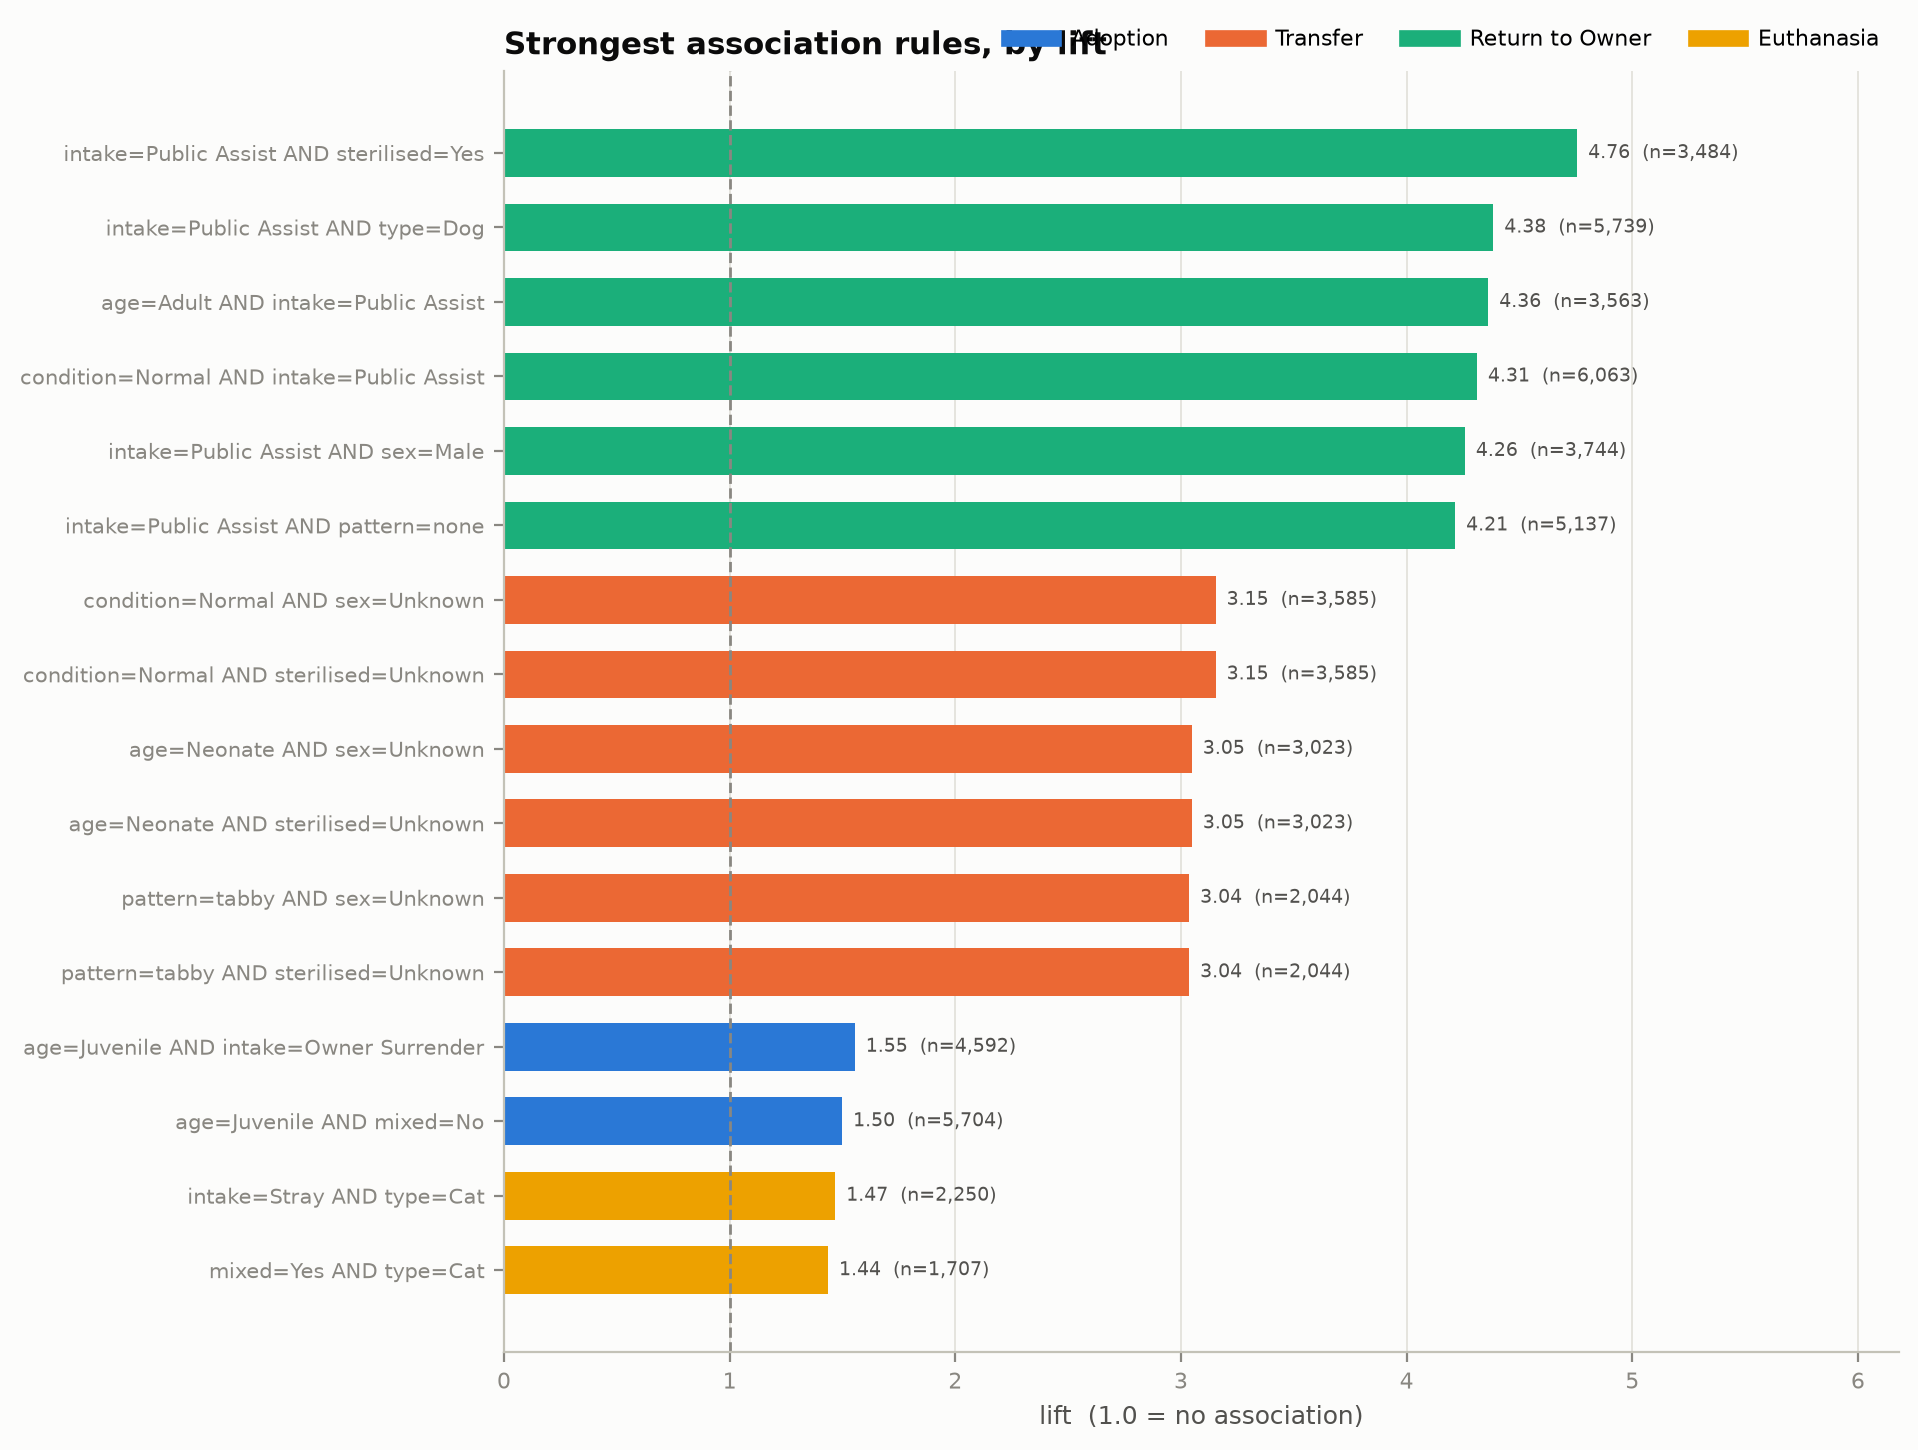
\includegraphics[width=0.95\textwidth]{02-rules-lift.png}
\caption{Strongest mined rules. The dominant pattern is \texttt{intake=Public
Assist} $\rightarrow$ \texttt{Return to Owner} at a lift above 4: animals
brought in through the public-assist route are usually lost pets whose owners
are already looking for them.}
\end{figure}

A useful incidental finding: Apriori surfaced that \texttt{sex=Unknown} and
\texttt{sterilised=Unknown} are perfectly correlated, because both derive from a
single ``Unknown'' value in the source field. Rule mining exposed a redundancy in
our own encoding.

\subsection{Apriori against FP-Growth}

\begin{center}
\begin{tabular}{@{}R{2.6cm}R{2.4cm}R{2.6cm}R{2.2cm}R{2.0cm}@{}}
\toprule
\textbf{transactions} & \textbf{itemsets} & \textbf{Apriori (s)} &
\textbf{FP-Growth (s)} & \textbf{speed-up} \\
\midrule
20{,}000  & 4{,}503 & 1.77  & 1.78 & 0.99$\times$ \\
50{,}000  & 4{,}494 & 7.26  & 3.32 & 2.19$\times$ \\
100{,}000 & 4{,}440 & 17.21 & 5.17 & 3.33$\times$ \\
162{,}461 & 4{,}516 & 44.45 & 8.80 & \textbf{5.05}$\times$ \\
\bottomrule
\end{tabular}
\end{center}

The itemsets are identical; only the cost differs. Apriori rescans the database
once per candidate level, so its runtime climbs with the transaction count,
while FP-Growth builds its tree in two passes and stays comparatively flat. At
20{,}000 transactions the two are indistinguishable --- the crossover is
visible, which is a more honest result than a blanket claim that FP-Growth wins.

Absolute timings vary with machine load between runs; across repeated runs on
this hardware Apriori took between 44\,s and 89\,s at the full 162{,}461
transactions. The stable findings are the \emph{shape} --- Apriori growing
roughly linearly in $n$ while FP-Growth grows far more slowly --- and the
speed-up ratio, which reached 4.0$\times$ to 5.1$\times$ at full scale across
runs. Readers should reproduce rather than cite the seconds.

\subsection{Classification}
\label{sec:classification}

\begin{center}
\small
\begin{tabular}{@{}L{4.6cm}R{1.9cm}R{1.8cm}R{2.3cm}R{1.8cm}R{1.5cm}@{}}
\toprule
\textbf{Model} & \textbf{train rows} & \textbf{accuracy} & \textbf{balanced acc.}
& \textbf{macro F1} & \textbf{MCC} \\
\midrule
\multicolumn{6}{@{}l}{\textit{Random stratified split}} \\
Decision Tree               & 64{,}000 & 0.417 & \textbf{0.463} & 0.329 & 0.261 \\
Naive Bayes (Bernoulli)     & 64{,}000 & 0.493 & 0.387 & 0.358 & 0.260 \\
KNN ($k$=15)                & 19{,}999 & 0.592 & 0.322 & 0.326 & 0.298 \\
SVM (linear)                & 60{,}000 & 0.578 & 0.441 & \textbf{0.388} & 0.346 \\
SVM (RBF)                   & 10{,}001 & 0.509 & 0.447 & 0.374 & 0.310 \\
Neural Net (MLP, backprop)  & 64{,}000 & \textbf{0.628} & 0.373 & 0.382 & \textbf{0.375} \\
\midrule
\multicolumn{6}{@{}l}{\textit{Temporal holdout: train $\le$ 2021, test $\ge$ 2022}} \\
Decision Tree               & 62{,}157 & 0.418 & 0.421 & 0.302 & 0.222 \\
Naive Bayes (Bernoulli)     & 62{,}157 & 0.434 & 0.383 & 0.307 & 0.186 \\
KNN ($k$=15)                & 20{,}000 & 0.619 & 0.319 & 0.319 & 0.239 \\
SVM (linear)                & 60{,}000 & 0.585 & 0.439 & 0.364 & 0.308 \\
SVM (RBF)                   & 10{,}000 & 0.485 & 0.426 & 0.330 & 0.261 \\
Neural Net (MLP, backprop)  & 62{,}157 & 0.646 & 0.379 & \textbf{0.373} & 0.331 \\
\bottomrule
\end{tabular}
\end{center}

\textbf{Accuracy is the wrong number.} The two models with the best accuracy ---
the MLP at 0.628 and KNN at 0.592 --- have the \emph{worst} balanced accuracy,
0.373 and 0.322. They are predicting the majority class and being rewarded for
it. The decision tree, trained with balanced class weights, has the best
balanced accuracy at 0.463 and the second-worst accuracy at 0.417.

\begin{figure}[htbp]
\centering
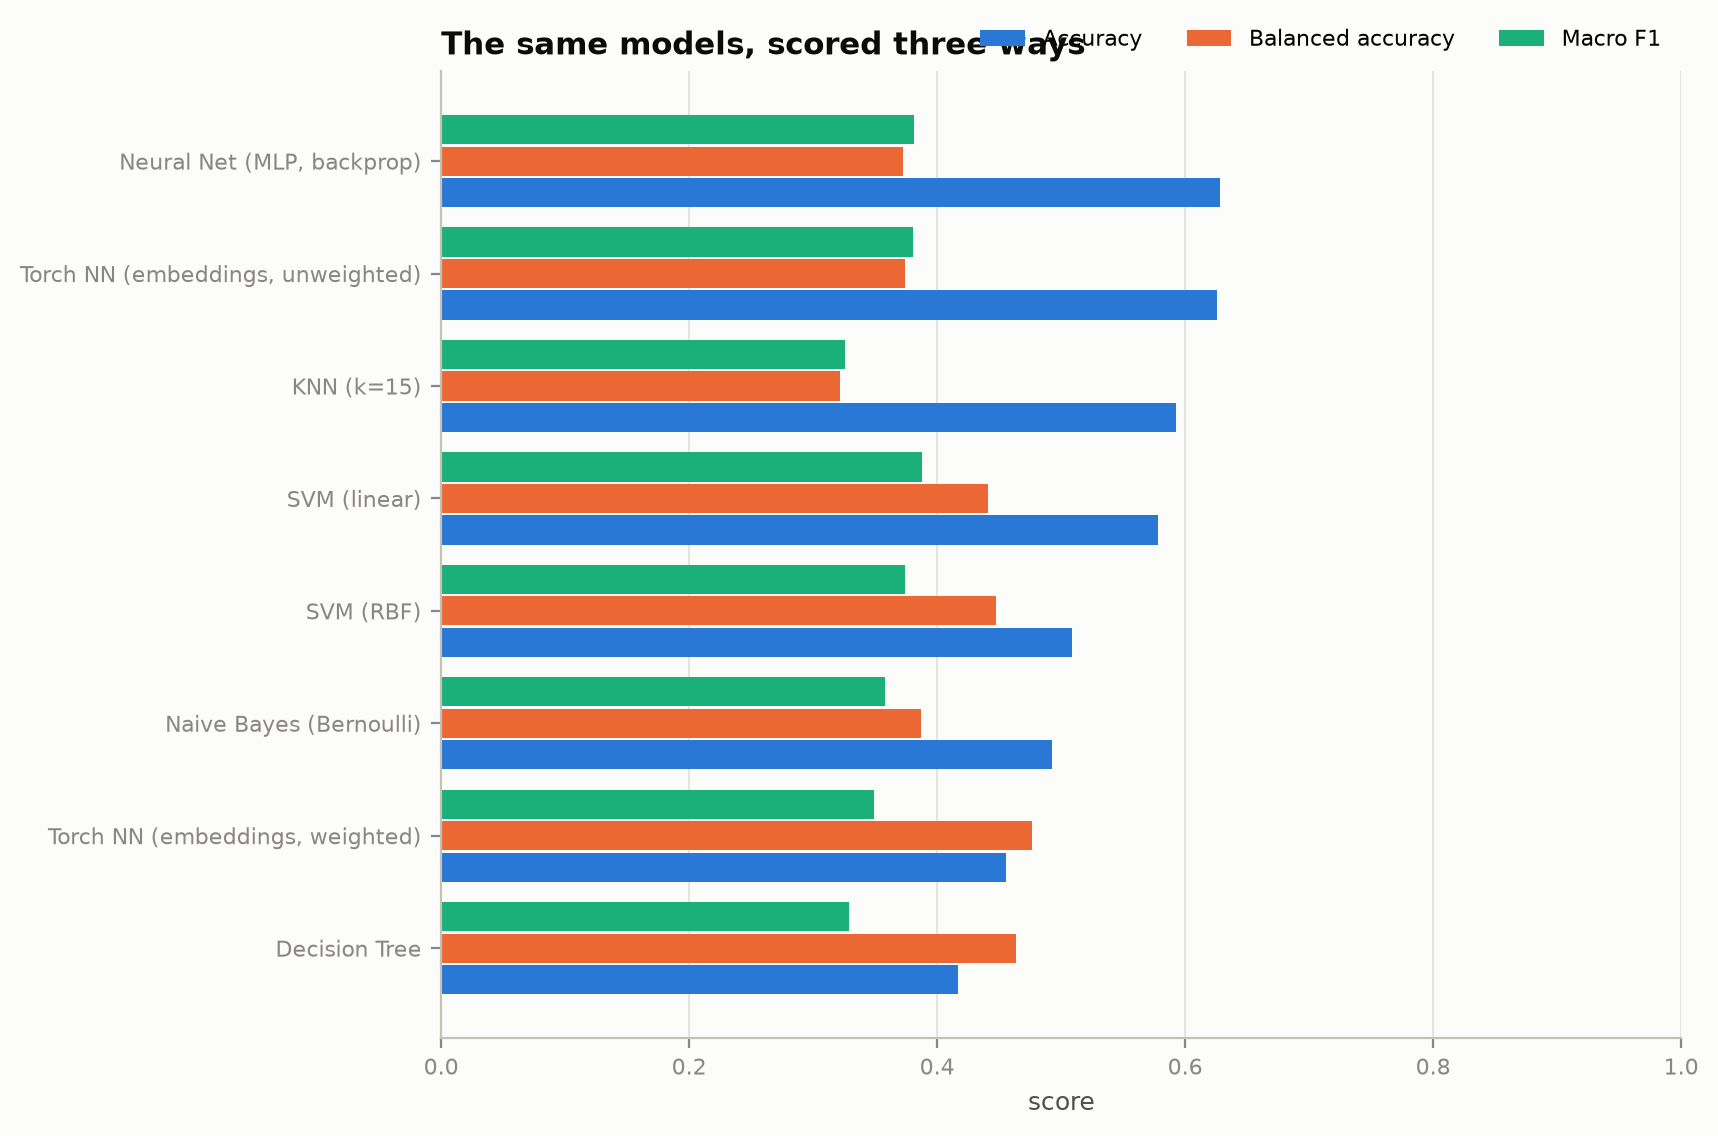
\includegraphics[width=0.85\textwidth]{05-accuracy-trap.png}
\caption{The same six models scored three ways. The ordering changes almost
completely between accuracy and balanced accuracy.}
\end{figure}

\textbf{Honest evaluation costs accuracy that was never there.} Mean MCC falls
from \textbf{0.308} under the random split to \textbf{0.258} under the temporal
holdout, a 16\,\% relative drop, and \emph{every} model degrades. Naive Bayes
loses the most (0.260 $\rightarrow$ 0.186). Interestingly the MLP's raw accuracy
\emph{rises} under the temporal split (0.628 $\rightarrow$ 0.646) while its MCC
falls --- the later period is more concentrated in the majority class, so
predicting it blindly scores better.

\begin{figure}[htbp]
\centering
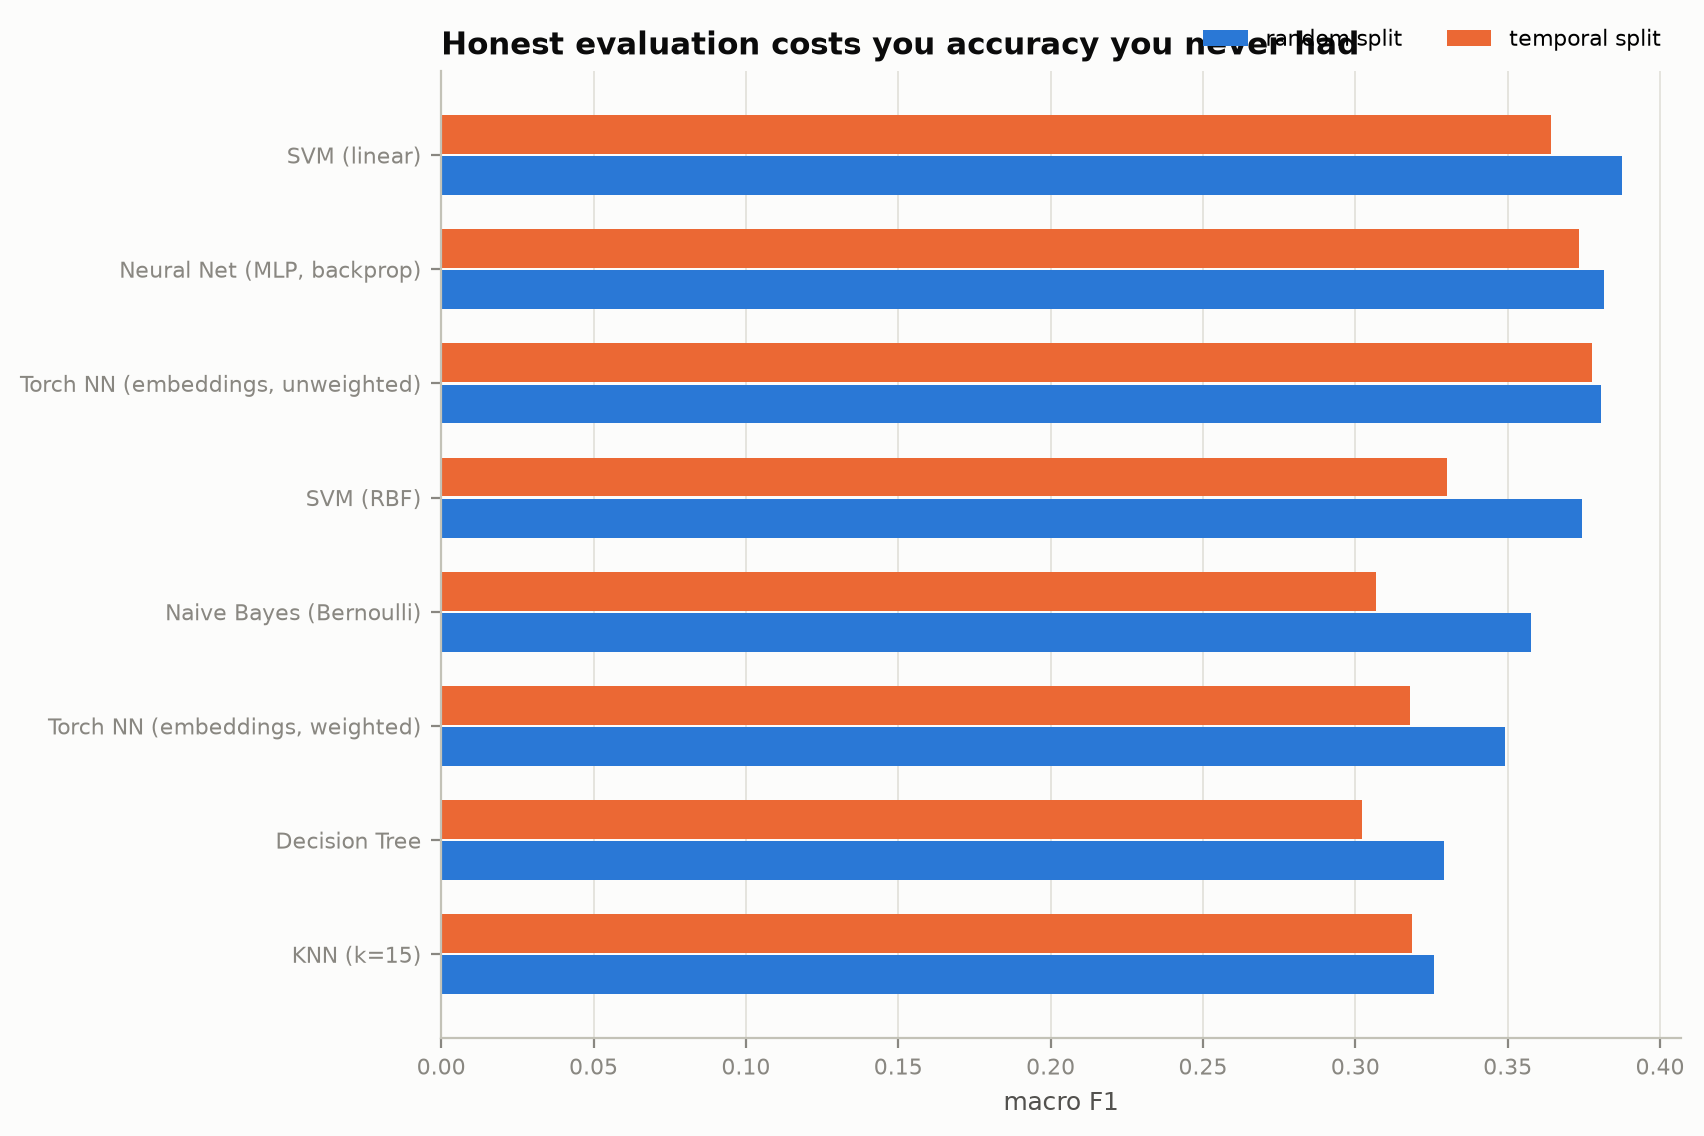
\includegraphics[width=0.78\textwidth]{04-protocol-comparison.png}
\caption{Macro F1 under both protocols. The random split is the optimistic one
for every model.}
\end{figure}

\subsection{A neural network in PyTorch, and why one was needed}
\label{sec:torch}

\texttt{MLPClassifier} is already a feedforward network trained by
backpropagation, so a second neural network needs a justification beyond
novelty. There are two, and both are things scikit-learn cannot do:

\textbf{1. A class-weighted loss.} \texttt{MLPClassifier} has no
\texttt{class\_weight} parameter. That is precisely why it posts the best
accuracy in the study (0.628) and nearly the worst balanced accuracy (0.373):
with Adoption at 51.6\,\% of records it has no mechanism to resist predicting
the majority class. \texttt{nn.CrossEntropyLoss(weight=\ldots)} supplies one.

\textbf{2. Learned embeddings.} One-hot encoding places the 50 breed groups in
50 mutually orthogonal directions, so Labrador is exactly as far from Golden
Retriever as from Siamese. An embedding layer learns a dense vector per category
from the outcome signal instead. There is no scikit-learn equivalent.

\begin{center}
\small
\begin{tabular}{@{}L{6.4cm}R{1.9cm}R{2.3cm}R{1.9cm}R{1.5cm}@{}}
\toprule
\textbf{Model (random split)} & \textbf{accuracy} & \textbf{balanced acc.} &
\textbf{macro F1} & \textbf{MCC} \\
\midrule
Neural Net (sklearn MLP, one-hot) & 0.628 & 0.373 & 0.382 & 0.375 \\
Torch NN (embeddings, unweighted) & 0.626 & 0.374 & 0.381 & 0.373 \\
Torch NN (embeddings, weighted)   & 0.455 & \textbf{0.477} & 0.349 & 0.284 \\
\bottomrule
\end{tabular}
\end{center}

The \textbf{unweighted} torch network reproduces the sklearn MLP to within
0.003 on every single metric --- accuracy 0.626 against 0.628, balanced accuracy
0.374 against 0.373, macro F1 0.381 against 0.382. That near-identity is the
control, and it is worth more than a headline number: it confirms the
implementation is sound rather than accidentally different, and it shows that
the embeddings alone buy essentially nothing on this data. Eleven low-cardinality
categorical fields simply do not contain the structure that embeddings exist to
capture.

The \textbf{weighted} network is where the gain is. Accuracy falls from 0.626 to
0.455 while balanced accuracy rises from 0.374 to \textbf{0.477}, the highest of
any model in the study (the next best is the decision tree at 0.463). It is the
only model here with a dial between the two.

Honesty requires noting the cost: weighting \emph{lowers} macro F1, from 0.381
to 0.349, and the best macro F1 overall still belongs to the linear SVM at
0.388. Over-predicting the rare classes raises their recall at the expense of
their precision, and macro F1 charges for both. Which setting is correct depends
on what the shelter wants --- a screening tool that must not miss at-risk
animals should accept the false positives.

\begin{figure}[htbp]
\centering
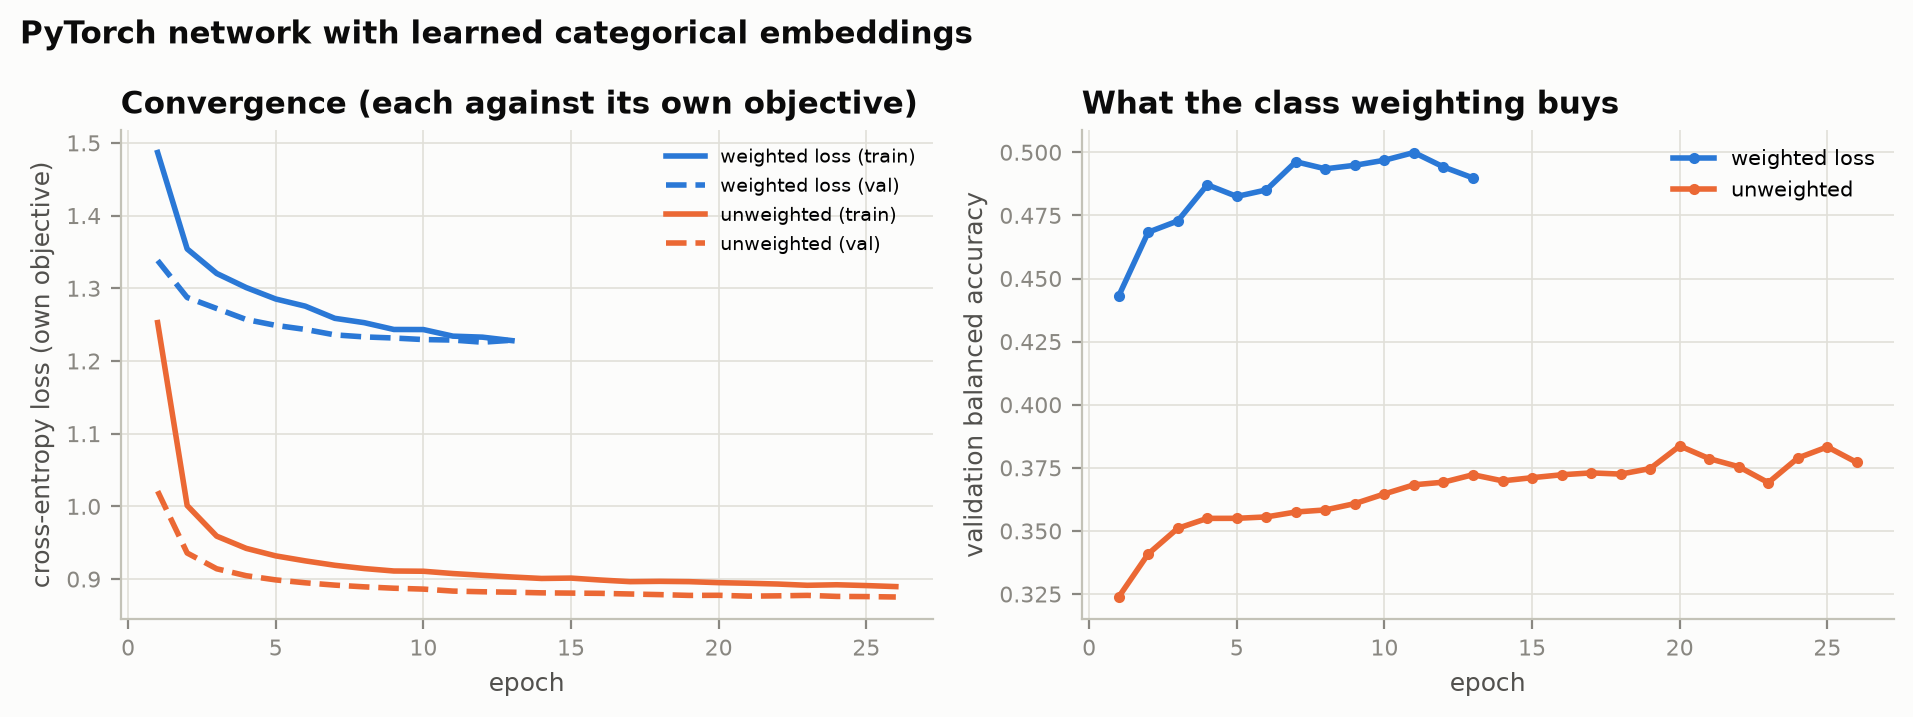
\includegraphics[width=0.95\textwidth]{13-torch-training.png}
\caption{Left: convergence. The two variants optimise \emph{different}
objectives, so their absolute heights are not comparable --- each solid curve is
meaningful only against its own dashed validation twin, and the weighted model's
growing gap after epoch 10 is overfitting. Right: validation balanced accuracy,
where the two \emph{are} comparable, and the weighting is worth roughly ten
points.}
\end{figure}

The training loop is written out explicitly --- \texttt{zero\_grad},
forward pass, loss, \texttt{backward()}, \texttt{step()} --- rather than hidden
behind a \texttt{.fit()} call, which is the part of the syllabus it is meant to
demonstrate. Training takes under a minute on CPU; no GPU is used anywhere in
this project.

\subsection{Clustering}

\begin{center}
\small
\begin{tabular}{@{}L{6.2cm}R{1.6cm}R{1.5cm}R{1.5cm}L{3.4cm}@{}}
\toprule
\textbf{Algorithm} & \textbf{clusters} & \textbf{ARI} & \textbf{NMI} &
\textbf{dissimilarity} \\
\midrule
K-Means (one-hot, $k$=8)          & 8  & 0.011 & 0.041 & Euclidean on one-hot \\
K-Medoids (Hamming, $k$=8)        & 8  & 0.018 & 0.044 & Hamming \\
Hierarchical (complete, Hamming)  & 8  & 0.031 & 0.048 & Hamming \\
Hierarchical (average, Hamming)   & 8  & \textbf{0.037} & \textbf{0.065} & Hamming \\
Hierarchical (ward, one-hot)      & 8  & 0.024 & 0.062 & Euclidean on one-hot \\
DBSCAN ($\le$1 attribute differs) & 7  & 0.031 & 0.065 & Hamming \\
OPTICS (Hamming, $\xi$)           & 16 & 0.000 & 0.049 & Hamming \\
\bottomrule
\end{tabular}
\end{center}

\textbf{Clustering does not recover the outcome classes.} Every ARI sits between
0.000 and 0.037, which is close to chance. We report this rather than tune it
away: animals that look alike on intake do not share a fate, which is itself
informative --- it means outcome is not simply a function of the animal's
visible attributes.

Within that, the three Hamming-based methods outperform K-Means on one-hot data
(0.018--0.037 against 0.011), which is the expected direction given
Section~\ref{sec:hamming}, though the margin is small enough that we would not
rest an argument on it alone.

\subsection{The atypicality test}

The headline unsupervised result. DBSCAN and OPTICS label low-density points as
noise --- animals whose attribute combination is unusual. No labels are used to
find them; labels only score them afterwards.

\begin{center}
\begin{tabular}{@{}L{5.6cm}R{1.8cm}R{2.4cm}R{2.6cm}R{1.6cm}@{}}
\toprule
\textbf{Algorithm} & \textbf{noise $n$} & \textbf{euth.\ noise} &
\textbf{euth.\ clustered} & \textbf{ratio} \\
\midrule
DBSCAN ($\le$1 attribute differs) & 1{,}221 & 5.65\,\% & 2.20\,\% & \textbf{2.57$\times$} \\
DBSCAN ($\le$2 attributes differ) & 61      & 14.75\,\% & 2.78\,\% & 5.31$\times$ \\
OPTICS (Hamming, $\xi$)           & 1{,}763 & 4.03\,\% & 1.29\,\% & \textbf{3.11$\times$} \\
\bottomrule
\end{tabular}
\end{center}

Two independent density algorithms agree: atypical animals are euthanised at
between two and a half and three times the rate of animals that fall inside a
cluster, and are adopted less often (46.5\,\% against 52.9\,\% for DBSCAN).

\begin{figure}[htbp]
\centering
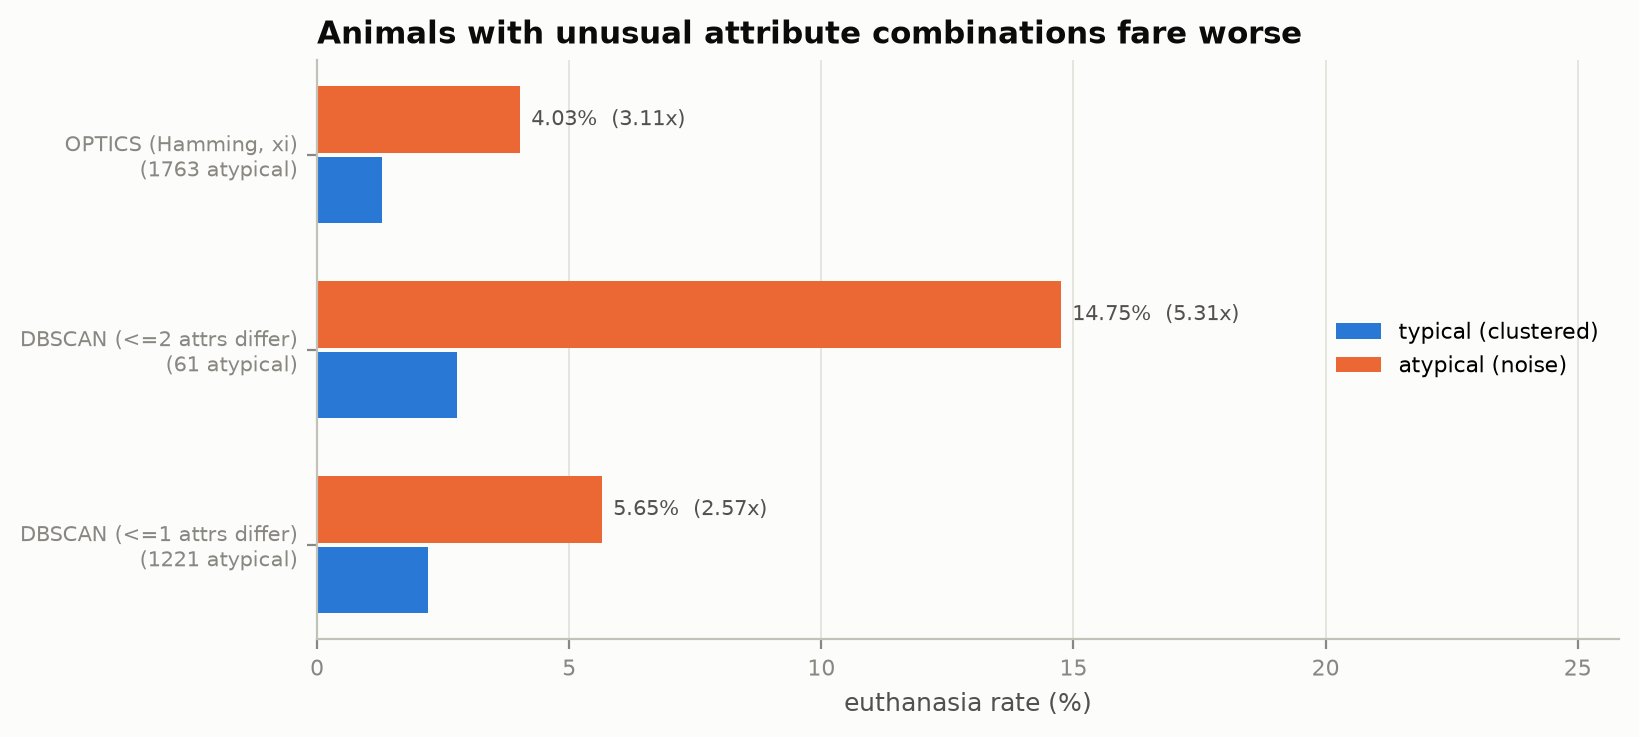
\includegraphics[width=0.86\textwidth]{08-atypicality.png}
\caption{Euthanasia rate for animals inside a cluster against those labelled
noise. Sample sizes are printed on the axis so the reader can judge the
61-animal row for themselves.}
\end{figure}

A fourth configuration (DBSCAN at $\le$3 attributes) produced exactly
\textbf{one} noise point and duly reported a ``100\,\% euthanasia rate'' at
34.7$\times$ lift. The pipeline marks any noise group below 30 animals
unreliable and excludes it from figures and the summary. Without that guard this
would have been the most eye-catching number in the report and entirely
meaningless.

\subsection{Association rules against decision tree paths}
\label{sec:cmp}

Both methods search the same data for structure. Apriori enumerates frequent
attribute combinations exhaustively above a support floor; a decision tree
greedily partitions on information gain. Do they find the same thing?

\textbf{On rules, largely yes.} Of 45 tree leaves, \textbf{30 (66.7\,\%)} are
covered by a mined rule predicting the same outcome. Of the fifteen that are
not, one relies on negation --- which positive-item Apriori cannot express at
all --- and seven fall below Apriori's support floor.

\textbf{On attributes, not at all.}

\begin{center}
\begin{tabular}{@{}L{3.4cm}R{3.0cm}R{3.0cm}@{}}
\toprule
\textbf{Attribute} & \textbf{tree share} & \textbf{Apriori share} \\
\midrule
intake condition & \textbf{32.1\,\%} & 5.8\,\% \\
intake type      & 18.3\,\% & 11.3\,\% \\
sterilised       & 16.4\,\% & 8.3\,\% \\
animal type      & 16.0\,\% & 9.7\,\% \\
age band         & 14.0\,\% & \textbf{15.1\,\%} \\
sex              & 1.8\,\% & 7.6\,\% \\
mixed breed      & 1.1\,\% & 5.5\,\% \\
\textbf{breed group} & \textbf{0.2\,\%} & 10.6\,\% \\
\textbf{colour group} & \textbf{0.1\,\%} & 12.0\,\% \\
colour pattern   & 0.0\,\% & 7.9\,\% \\
multicolour      & 0.0\,\% & 6.3\,\% \\
\bottomrule
\end{tabular}
\end{center}

Spearman rank correlation between the two rankings is \textbf{0.055} ---
effectively zero. The tree concentrates 96.9\,\% of its attention on five
attributes and \emph{never meaningfully splits on breed or colour}. Apriori
spreads evenly and reports breed and colour patterns freely.

\begin{figure}[htbp]
\centering
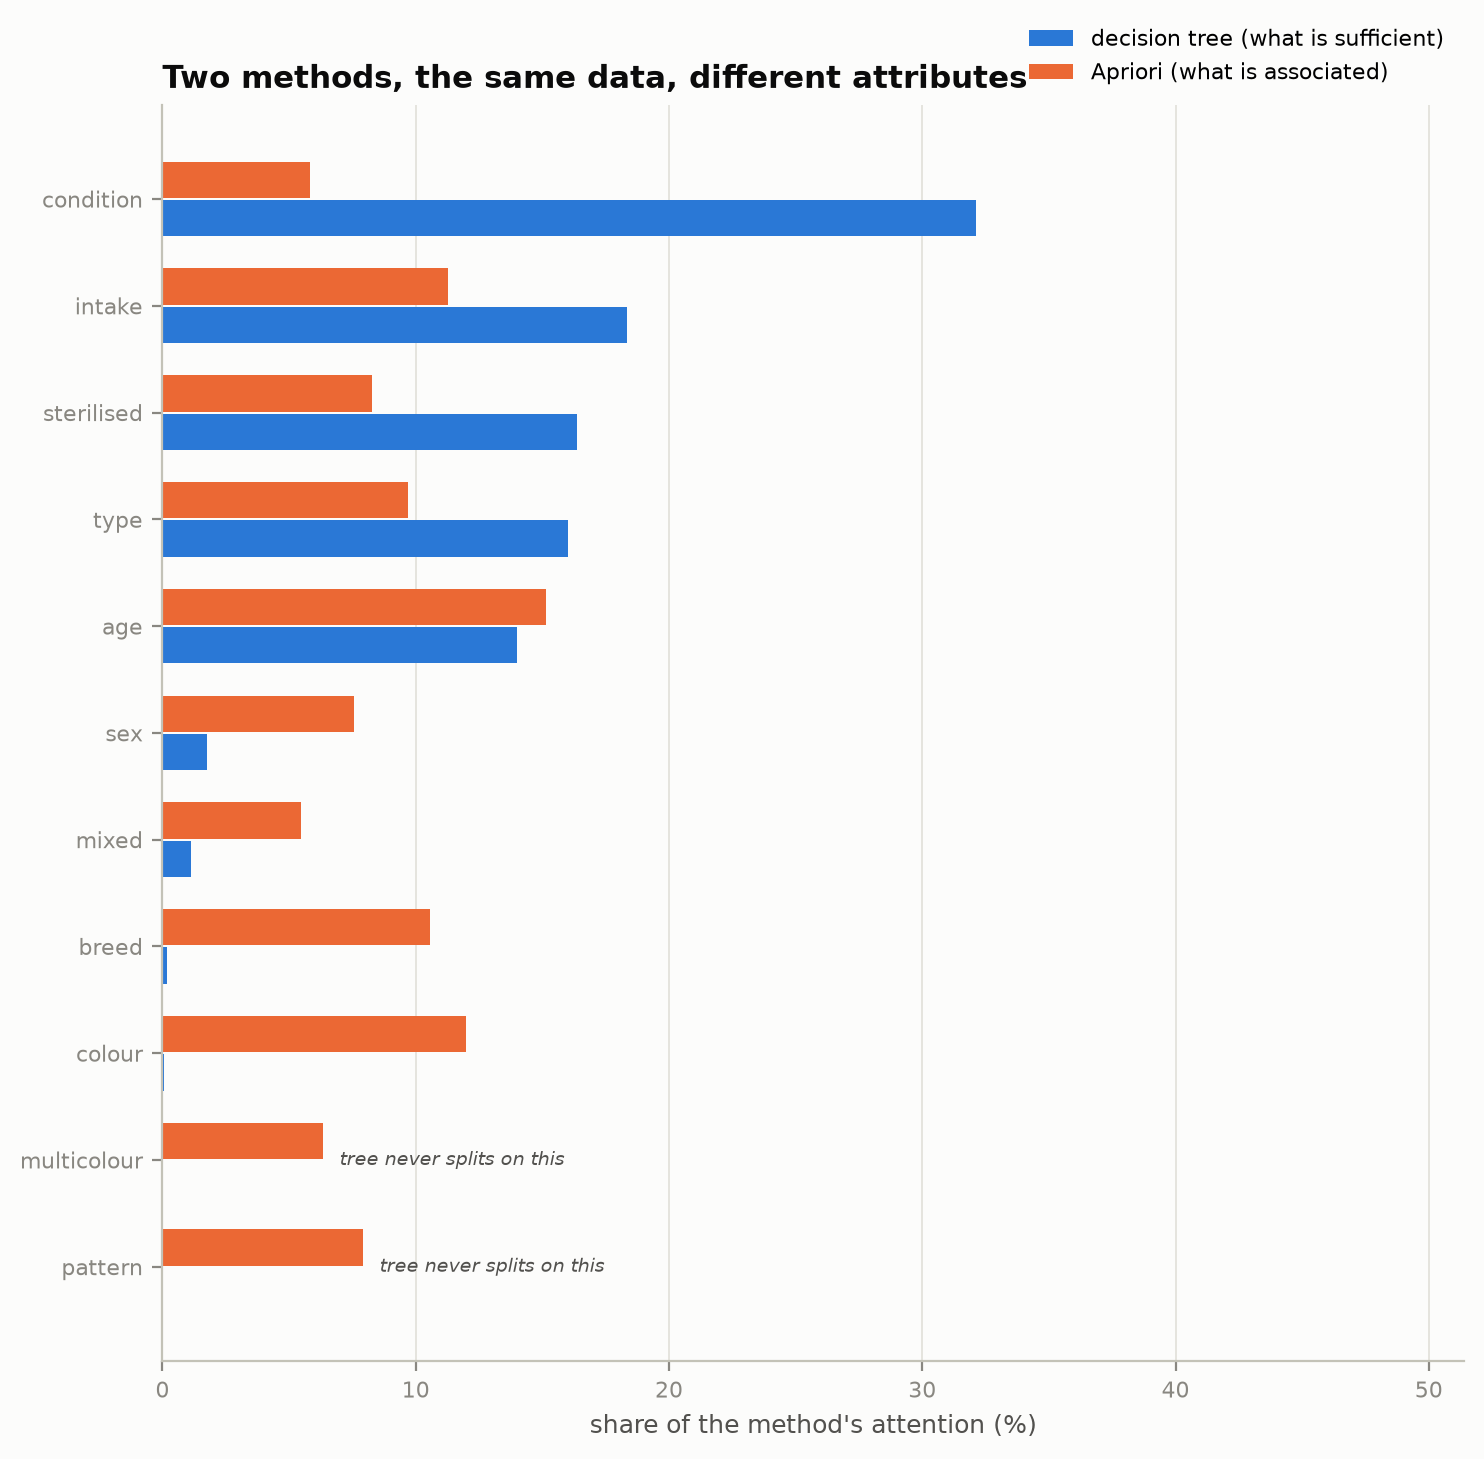
\includegraphics[width=0.84\textwidth]{12-field-ranking.png}
\caption{Where each method places its attention. The disagreement is the
finding, not an error.}
\end{figure}

This is not a contradiction. It is the difference between two questions. A
decision tree finds what is \textbf{sufficient}: once species, intake condition,
intake route and age are known, colour adds no information gain, so it is never
split on. Apriori finds what is \textbf{associated}, and colour genuinely is
associated. Section~\ref{sec:bias} reaches the same conclusion by a third,
entirely independent route.

\subsection{Attribute bias}
\label{sec:bias}

The question the project set out to answer. Confounding is the trap: black
animals are not distributed evenly across species, ages and intake routes, so a
raw comparison partly measures ``what kind of animal tends to be black''. We use
\textbf{direct standardisation} --- compute rates within (species $\times$ age
band $\times$ intake route) strata, then reweight to the whole population's
stratum mix.

\begin{center}
\small
\begin{tabular}{@{}L{5.4cm}R{1.5cm}R{2.0cm}R{1.9cm}R{2.3cm}@{}}
\toprule
\textbf{Claim} & \textbf{$n$} & \textbf{adoption gap} &
\textbf{median stay} & \textbf{euthanasia} \\
\midrule
Black cats vs other cats     & 15{,}898 & $-$2.25 pp  & 8.1 vs 7.1 d & 4.08 vs 3.56\,\% \\
Black dogs vs other dogs     & 25{,}118 & \textbf{+2.77 pp} & 6.1 vs 6.0 d & 2.09 vs 2.40\,\% \\
Pit bull type vs other dogs  & 16{,}531 & $-$4.34 pp  & \textbf{10.0 vs 5.3 d} & 4.35 vs 1.89\,\% \\
Senior vs non-senior dogs    & 10{,}019 & \textbf{$-$23.66 pp} & 4.0 vs 6.1 d & 5.50 vs 1.94\,\% \\
Senior vs non-senior cats    & 3{,}800  & $-$10.32 pp & 8.2 vs 7.2 d & \textbf{12.74 vs 3.15\,\%} \\
Mixed breed vs purebred dogs & 74{,}526 & +4.11 pp    & 6.0 vs 5.9 d & 2.36 vs 2.16\,\% \\
\bottomrule
\end{tabular}
\end{center}

\begin{figure}[htbp]
\centering
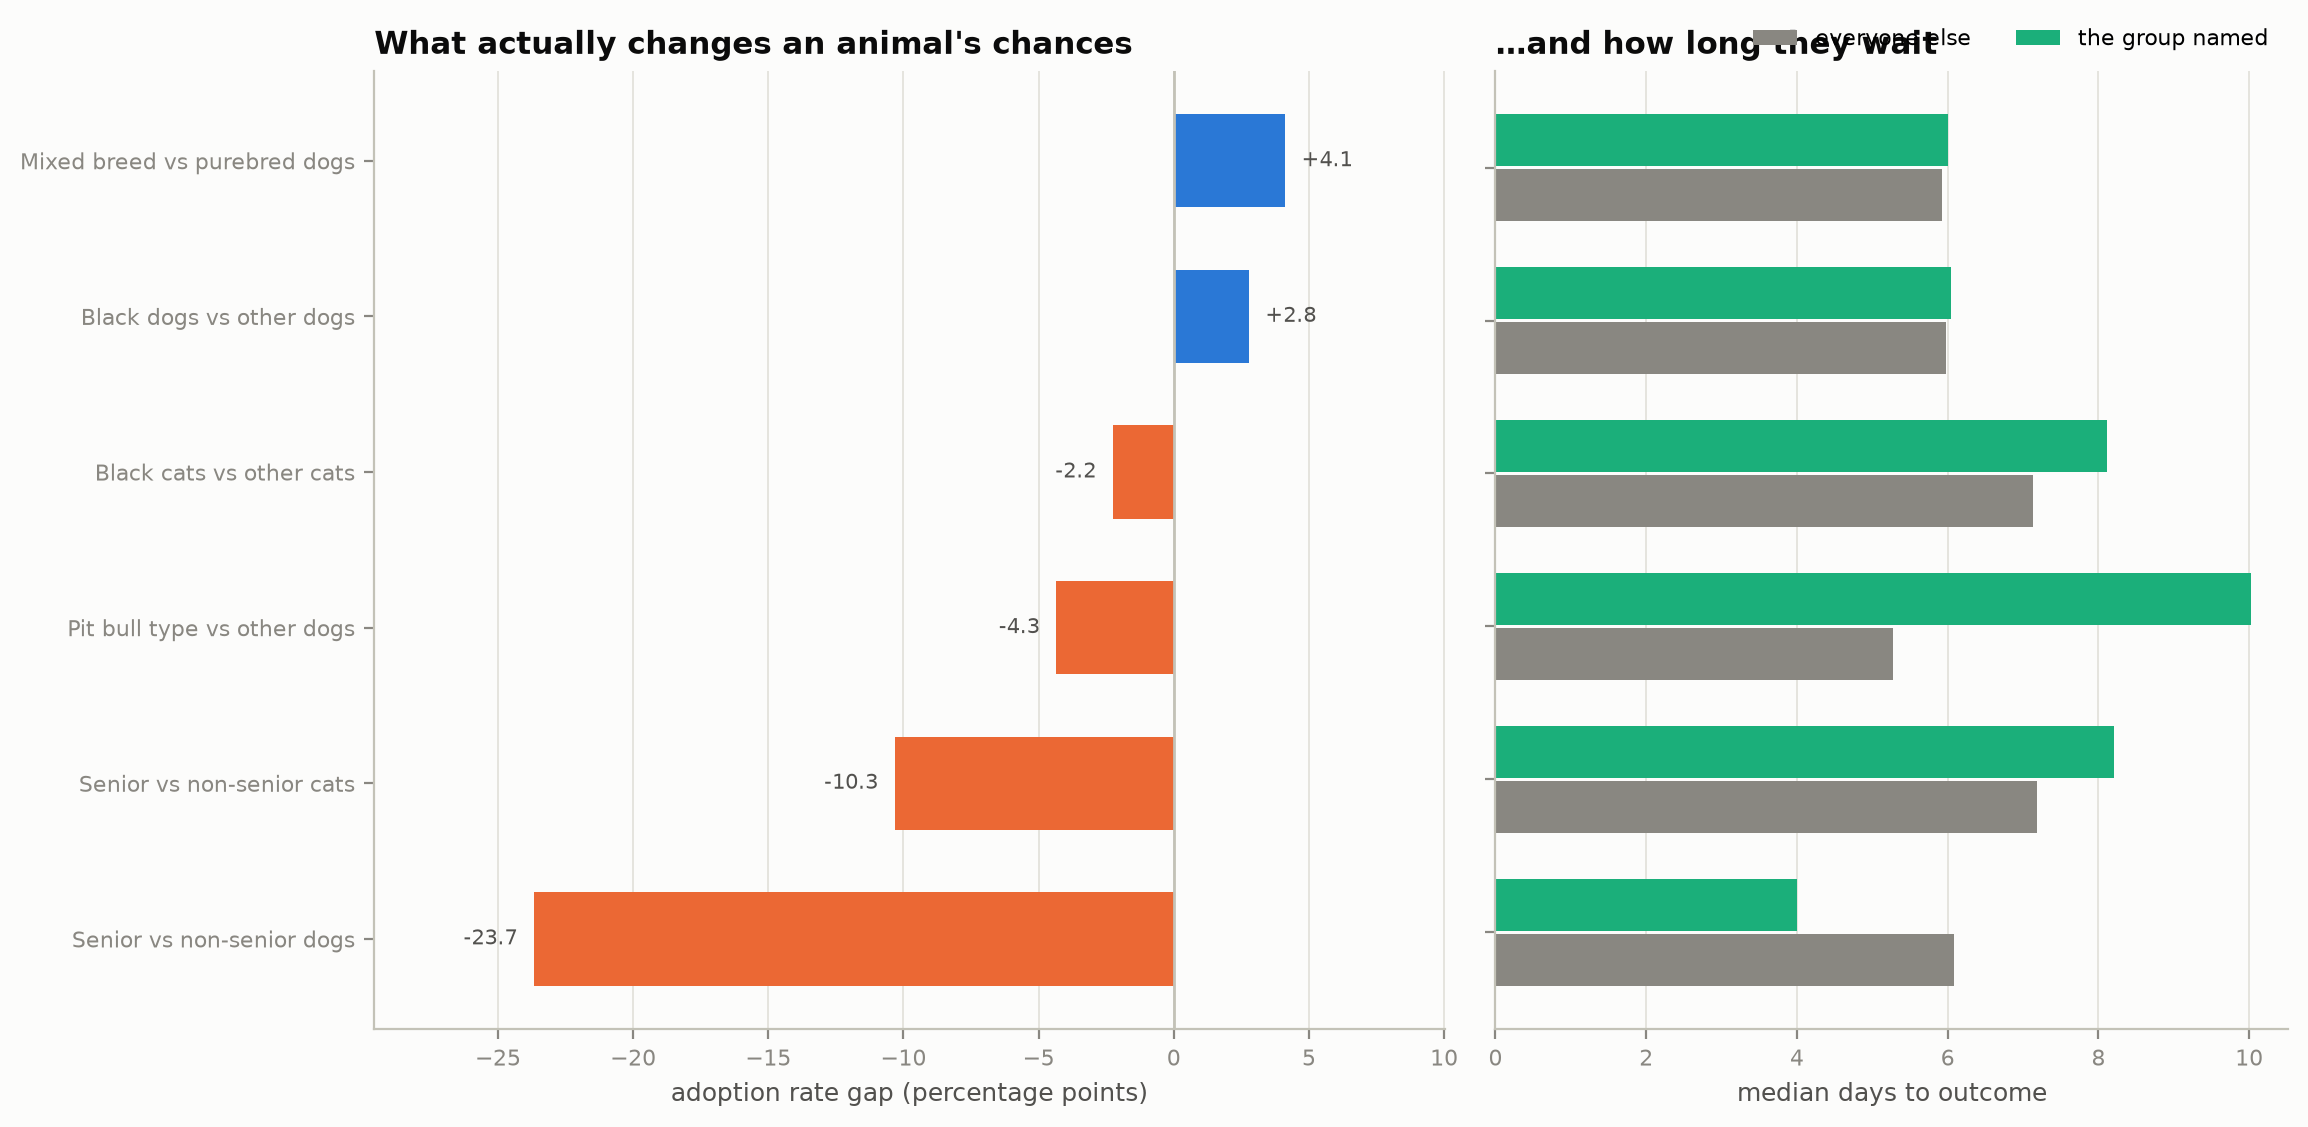
\includegraphics[width=\textwidth]{10-claims.png}
\caption{Adoption gap and waiting time for each claim. The trait that attracts
public attention is close to noise; the traits that do not are large.}
\end{figure}

\textbf{Black dog syndrome is not supported.} Black dogs are adopted
\emph{more} than other dogs and euthanised \emph{less}. Black cats are adopted
2.25 pp less and wait about one extra day --- a real but small effect. After
standardisation black sits mid-table at 51.6\,\% and \textbf{white} animals are
lowest at 49.5\,\%.

\textbf{Mixed-breed stigma is not visible either}; mixed dogs are adopted 4.11
pp \emph{more} than purebreds.

\textbf{Age is the dominant factor.} Senior dogs are adopted 23.66 pp less often
than non-seniors and euthanised at nearly three times the rate. Senior cats are
euthanised at \textbf{12.74\,\% against 3.15\,\%} --- a fourfold difference and
the single starkest number in the study. Their shorter median stay (4.0 days for
senior dogs) is not good news: they leave quickly because they leave by a
different exit.

\textbf{Breed label costs time more than it costs adoptions.} Pit bull type dogs
are adopted 4.34 pp less --- but wait a median of 10.0 days against 5.3, and are
euthanised at 4.35\,\% against 1.89\,\%.

\begin{figure}[htbp]
\centering
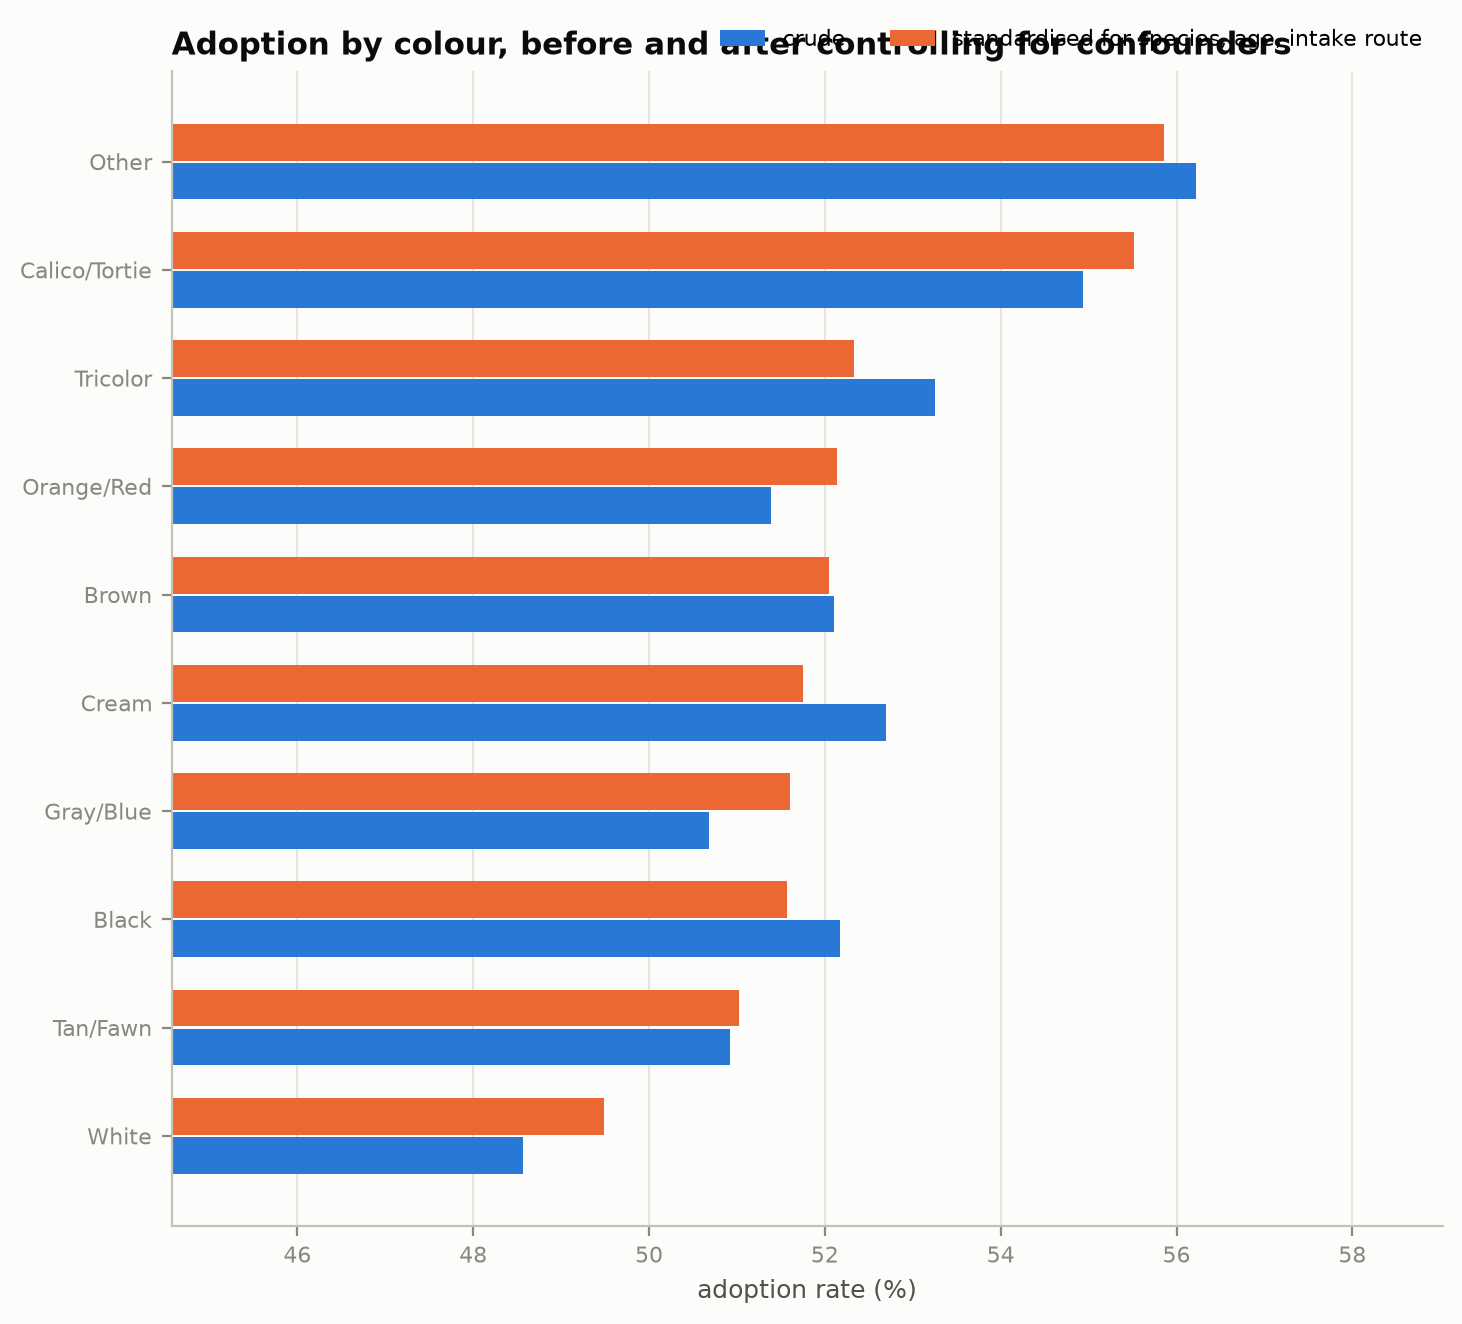
\includegraphics[width=0.8\textwidth]{11-colour-adjusted.png}
\caption{Adoption by colour before and after standardising for species, age band
and intake route. The adjustment moves every colour by less than one percentage
point: colour's apparent effect was small to begin with.}
\end{figure}

%% ==================================================================
\section{Discussion}

Three methods converge on the same conclusion about colour. Direct
standardisation shows the effect is small and that white, not black, is lowest.
The decision tree never splits on colour, because it adds no information once
species, condition and age are known. Apriori does report colour rules, because
colour \emph{is} associated --- but association without sufficiency is exactly
what confounding looks like. Agreement across a descriptive adjustment, a greedy
supervised partition and an exhaustive unsupervised search is stronger evidence
than any one of them.

The practical implication inverts the usual shelter advice. Effort spent
photographing black animals more flatteringly is effort spent on a 2 pp effect
in cats and a negative effect in dogs. The same effort directed at senior
animals addresses a 23 pp gap and a fourfold euthanasia difference.

The atypicality result suggests a cheap triage signal. A shelter already records
every attribute used here at intake. Running DBSCAN over the recent intake
population and flagging the noise points identifies, with no labelled training
data and no model to maintain, a group with roughly triple the baseline
euthanasia rate.

%% ==================================================================
\section{Limitations}

\begin{itemize}
  \item \textbf{One shelter, one city.} Austin operates an explicit no-kill
        policy; its 2.9\,\% euthanasia rate is far below the national average,
        and effects measured here may not transfer.
  \item \textbf{Association, not causation.} Standardisation controls the
        confounders we measured. Temperament, medical history and photograph
        quality are not in the data and are plausibly correlated with both
        colour and outcome.
  \item \textbf{Breed and colour are free text}, normalised by rules we wrote.
        98.9\,\% of records reach a named breed group; the mapping is published
        with the code and is arguable.
  \item \textbf{Clustering subsamples.} The metric-based algorithms see 6{,}000
        of 162{,}461 records because a full dissimilarity matrix would be
        $\sim$105\,GB. The classification results use up to 64{,}000.
  \item \textbf{Clustering does not recover outcomes} (ARI $\le$ 0.037). The
        clusters are real groupings of animals; they are simply not groupings of
        fate.
  \item \textbf{``Pit bull'' is a label, not a breed.} It is assigned by staff on
        visual inspection and is known to be unreliable, so the pit bull result
        measures the effect of the \emph{label} --- which is arguably the more
        relevant quantity anyway.
\end{itemize}

%% ==================================================================
\section{Conclusion}

Using only the algorithms taught in this course, on a public dataset of 162{,}461
shelter outcomes, we find that the attribute bias people believe in is
measurably absent and the biases they do not discuss are large. Black dogs are
adopted more than other dogs; senior cats are euthanised at four times the rate
of younger ones.

Density-based clustering identifies a materially at-risk group without any
labels, at roughly three times the baseline euthanasia rate. Association rules
and decision trees agree on two thirds of their rules while disagreeing
completely on which attributes matter, and that disagreement --- sufficiency
against association --- turns out to explain the colour result independently.

Honest temporal evaluation lowers every score we report. We report the lower
ones.

%% ==================================================================
\section*{Reproducing this report}
\addcontentsline{toc}{section}{Reproducing this report}

\begin{verbatim}
pip install -r requirements.txt
python run_all.py --quick     # ~6 min, end-to-end check
python run_all.py             # full run, ~18 min
python src/tool.py --type Dog --age Senior --intake "Owner Surrender"
\end{verbatim}

Every table and figure in this report is regenerated by \texttt{run\_all.py}
from the two public CSVs, which the loader downloads and caches on first run.

%% ==================================================================
\section*{References}
\addcontentsline{toc}{section}{References}

\begin{enumerate}[label={[\arabic*]}]
  \item City of Austin, ``Austin Animal Center Outcomes'' and ``Austin Animal
        Center Intakes,'' City of Austin Open Data Portal. [Online]. Available:
        \url{https://data.austintexas.gov/}
  \item R. Agrawal and R. Srikant, ``Fast Algorithms for Mining Association
        Rules,'' in \emph{Proc. 20th Int. Conf. Very Large Data Bases (VLDB)},
        1994, pp.~487--499.
  \item J. Han, J. Pei, and Y. Yin, ``Mining Frequent Patterns without Candidate
        Generation,'' in \emph{Proc. ACM SIGMOD Int. Conf. Management of Data},
        2000, pp.~1--12.
  \item M. Ester, H.-P. Kriegel, J. Sander, and X. Xu, ``A Density-Based
        Algorithm for Discovering Clusters in Large Spatial Databases with
        Noise,'' in \emph{Proc. 2nd Int. Conf. KDD}, 1996, pp.~226--231.
  \item M. Ankerst, M. M. Breunig, H.-P. Kriegel, and J. Sander, ``OPTICS:
        Ordering Points To Identify the Clustering Structure,'' in \emph{Proc.
        ACM SIGMOD}, 1999, pp.~49--60.
  \item L. Kaufman and P. J. Rousseeuw, \emph{Finding Groups in Data: An
        Introduction to Cluster Analysis}. New York: Wiley, 1990.
  \item Z. Huang, ``Extensions to the $k$-Means Algorithm for Clustering Large
        Data Sets with Categorical Values,'' \emph{Data Mining and Knowledge
        Discovery}, vol.~2, no.~3, pp.~283--304, 1998.
  \item F. Pedregosa \emph{et al.}, ``Scikit-learn: Machine Learning in
        Python,'' \emph{JMLR}, vol.~12, pp.~2825--2830, 2011.
  \item S. Raschka, ``MLxtend,'' \emph{Journal of Open Source Software},
        vol.~3, no.~24, p.~638, 2018.
\end{enumerate}

\vspace{6pt}
\noindent\footnotesize\emph{Note to the group: references [2]--[9] are the
primary sources for the algorithms and tools used, and should be verified
against your own library versions. Before submission add two or three domain
references on shelter adoption outcomes and ``black dog syndrome'' from the
animal-welfare literature --- \emph{Anthrozo\"os} and the \emph{Journal of
Applied Animal Welfare Science} both publish on this --- and check every
citation yourself.}

\end{document}
